\documentclass{article}
\usepackage{url}
\usepackage{amsmath,bm}%
\usepackage{amsfonts}%
\pagestyle{empty}
\setlength{\textwidth}{7in}
\setlength{\oddsidemargin}{-.5in}
\setlength{\evensidemargin}{-.5in}
\setlength{\topmargin}{-.75in}
\setlength{\textheight}{9.4in}

\newcommand{\beaa}{\begin{eqnarray*}}
\newcommand{\eeaa}{\end{eqnarray*}}
\newcommand{\bea}{\begin{eqnarray}}
\newcommand{\eea}{\end{eqnarray}}
\def\E{\mathop{\rm E\,}\nolimits}
\def\Var{\mathop{\rm Var\,}\nolimits}
\def\Cov{\mathop{\rm Cov\,}\nolimits}
\def\Corr{\mathop{\rm Corr\,}\nolimits}
\def\logit{\mathop{\rm logit\,}\nolimits}
\newcommand{\eid}{{\stackrel{\cal{D}}{=}}}
\newcommand{\cip}{{\stackrel{{P}}{\to}}}
\def\bR{\mathbb{R}}     % real line

\usepackage{Sweave}
\begin{document}

\begin{center}
{\bf STAT 515}

{\bf Homework \#10 WITH SOLUTIONS}

\end{center}

\begin{enumerate}

  \item We wish to approximate $\mu=P(X>4.5)$ where $X\sim N(0,1)$. Suppose that
  $q(x)$ is a normal density with mean $k$, and suppose that $X_1, \ldots, X_n$
  is a simple random sample from $q(\cdot)$.
  
    \begin{enumerate}
    
      \item Show that 
      \[
      \tilde\mu = \frac{ \frac1n \sum_{i=1}^n I\{X_i>4.5\} \exp\{
      (X_i-k)^2/2-X_i^2/2 \} }
      { \frac1n \sum_{i=1}^n \exp\{ (X_i-k)^2/2-X_i^2/2 \} }
      \]
      is a consistent estimator of $\mu$. (To do this, it's enough to show that
      the true mean of the numerator divided by the true mean of the denominator
      equals $\mu$.)
      \begin{quotation}{\bf Solution:}
      For the numerator, we obtain for $X\sim N(k, 1)$,
      \begin{eqnarray*}
      E \left[ I\{X_i>4.5\} \exp\{ (X-k)^2/2-X^2/2 \} \right]  &=& 
      \int_{4.5}^\infty \exp\{ (x-k)^2/2-x^2/2 \} \frac{1}{\sqrt{2\pi}} \exp\{-(x-k)^2/2 \} \, dx \\
      &=& \int_{4.5}^\infty \frac{1}{\sqrt{2\pi}} \exp\{-x^2/2 \}  \, dx = \mu.
      \end{eqnarray*}
      A similar derivation shows that for the denominator,
      \[
      E \left[  \exp\{ (X-k)^2/2-X^2/2 \} \right]  =1.
      \]
      This means that $\hat\mu$ consists of a fraction in which the numerator
      is a sample mean whose true mean is $\mu$, and the denominator is a sample
      mean whose true mean is $1$.  This implies that $\hat\mu$ converges almost surely 
      to $\mu$.
      \end{quotation}
      
      \item Based on samples of size 100,000 from $q(\cdot)$, try using
      $\tilde\mu$ several times for $k=0$, $k=4.5$, and some intermediate values
      of $k$. What value of $k$ seems to give the most precise estimates?
      \begin{quotation}{\bf Solution:}
      Here is a function that returns 10 different estimates of $\mu$ based on a
      particular choice of $k$:
\begin{Schunk}
\begin{Sinput}
> f <- function(k, n=10) {
+   muhat <- 1:n
+   for (i in 1:n) {
+     x <- rnorm(1e5) + k
+     b <- exp((x-k)^2/2 - x^2/2)
+     a <- (x>4.5)*b
+     muhat[i] <- mean(a) / mean(b)
+   }
+   muhat
+ }
\end{Sinput}
\end{Schunk}
      Here are sample standard deviations for the 10 estimates for $k=0, 0.5, 1.0, \ldots, 4.5$:
\begin{Schunk}
\begin{Sinput}
> mu <- 1-pnorm(4.5)
> print(out <- sapply((0:9)/2, function(a) mean((f(a)-mu)^2)))
\end{Sinput}
\begin{Soutput}
 [1] 5.077211e-11 5.615992e-12 3.700880e-13 4.939637e-14 2.460070e-14
 [6] 5.623972e-14 3.708306e-13 2.690284e-13 2.135039e-12 2.495489e-11
\end{Soutput}
\begin{Sinput}
> ((0:9)/2)[which.min(out)] # Which value gave the smallest mean squared error?
\end{Sinput}
\begin{Soutput}
[1] 2
\end{Soutput}
\end{Schunk}
      So it appears that $k=2$ gives the best results of the ten values tested.
      \end{quotation}
      
      \item Use the delta-method derivation
      \[
      {\Var} \left( \frac{ \frac1n\sum_i A_i}{\frac1n\sum_i B_i} \right) \approx
      \frac{1}{n\mu_B^2}
      \begin{bmatrix}
      1 & \frac{-\mu_A}{\mu_B}
      \end{bmatrix}
      \begin{bmatrix}
      \sigma^2_A & \sigma_{AB} \\ \sigma_{AB} & \sigma^2_B
      \end{bmatrix}
      \begin{bmatrix}
      1 \\ \frac{-\mu_A}{\mu_B}
      \end{bmatrix}
      \]
      to estimate the variances of your $\tilde\mu$ estimators from part (b).
      (Use sample estimates of $\mu_A$, $\mu_B$, and the covariance matrix.) Do
      the variance estimates correspond with your experience in part (b)?
      \begin{quotation}{\bf Solution:}
      The following code modifies that of part (a) so that an estimator of the variance is returned
      along with $\hat\mu$:
\begin{Schunk}
\begin{Sinput}
> f2 <- function(k, n=1e5) {
+   x <- rnorm(n) + k
+   b <- exp((x-k)^2/2 - x^2/2)
+   a <- (x>4.5)*b
+   muhat <- mean(a) / mean(b)
+   v <- (z <- c(1, -muhat)) %*% cov(cbind(a,b)) %*% z / (n*mean(b)^2)
+   cbind(muhat=muhat, var=as.numeric(v))
+ }
\end{Sinput}
\end{Schunk}
     Now we may approximate the variance of the $\hat\mu$ estimator for various values of $k$:
\begin{Schunk}
\begin{Sinput}
> k <- (0:9)/2
> sapply(k, f2)[2,]  # Just print the variance estimates
\end{Sinput}
\begin{Soutput}
 [1] 0.000000e+00 9.597689e-13 6.786709e-13 9.026692e-14 2.803545e-14
 [6] 3.270997e-14 1.033955e-13 8.247448e-13 1.017039e-12 3.865547e-12
\end{Soutput}
\end{Schunk}
      The estimated variances here are of the same order of magnitude as 
      the mean squared errors in part (b), but we know that some of the
      approximations are not very good because the true variance must 
      always be smaller than the true MSE.  
      \end{quotation}
      
      \item Consider a modified estimator 
      \[
      \hat\mu = \frac1n \sum_{i=1}^n I\{X_i>4.5\} \exp\{ (X_i-k)^2/2-X_i^2/2 \},
      \]
      where once again $X_1, \ldots, X_n$ is a simple random sample from
      $q(\cdot)$. Verify that this estimator is a consistent estimator of $\mu$.
      (Again, merely show that the true mean of each summand equals $\mu$.)
      Using the best $k$ you found earlier, compare the estimated variance of
      $\tilde\mu$ with the estimated variance of $\hat\mu$ (the latter should
      not be hard to find). Which estimator, $\tilde\mu$ or $\hat\mu$, appears
      to be more precise?
      \begin{quotation}{\bf Solution:}
      Using $k=2$, we find:
\begin{Schunk}
\begin{Sinput}
> set.seed(12345) # Set seed so we can exactly replicate sample
> f2(2)[,2] # This is the ratio imp. samp. estimated variance
\end{Sinput}
\begin{Soutput}
         var 
2.911137e-14 
\end{Soutput}
\begin{Sinput}
> set.seed(12345) 
> x <- rnorm(1e5)+2
> var((x>4.5) * dnorm(x) / dnorm(x-2)) / 1e5 # Plain imp. samp. 
\end{Sinput}
\begin{Soutput}
[1] 2.361843e-14
\end{Soutput}
\end{Schunk}
      So it appears that the variance of the plain importance sampling estimator is smaller.
      NB:  This does not consider which estimator is more {\em accurate}, which is related
      to the bias.  However, since only the plain importance sampling estimate is theoretically
      unbiased, considering bias together with variance probably will not lead to a different
      conclusion. 
      
      Since part (c) suggests that the delta-method approximation of the variance might not be 
      very accurate, let us try to find a better variance estimator by measuring the sample variance
      of 1000 independent replicates of the ratio importance sampling estimator:
\begin{Schunk}
\begin{Sinput}
> var(f(2,n=1000))
\end{Sinput}
\begin{Soutput}
[1] 2.829011e-14
\end{Soutput}
\end{Schunk}
      We find fairly good agreement between this empirical estimate and the 
      asymptotic approximation based on the delta method.
      \end{quotation}
      
    \end{enumerate}

  \item Suppose that $X$ is a binomial random variable with parameters $n$ and
  $p$, where $p=e^\theta/(1+e^\theta)$ for some real-valued parameter $\theta$.
  The goal of this question will be to use ratio importance sampling to estimate
  the log-likelihood function $\ell(\theta) = \log P_\theta(X)$.
  
    \begin{enumerate}
    
      \item Show that the log-likelihood function may be written as
      \[
      \ell(\theta) = \theta X - \log c(\theta) + (\mbox{something not depending
      on $\theta$}),
      \] 
      and find the normalizing function $c(\theta)$.
      \begin{quotation}{\bf Solution:}
      Since $p=e^\theta/(1+e^\theta)$, the binomial mass function equals
      \[
      f_\theta(x) = 
      {n \choose x} \left( \frac{e^\theta}{1+e^\theta} \right)^x
      \left( \frac{1}{1+e^\theta} \right)^{n-x} =
      {n \choose x} e^{\theta x}
      \left( \frac{1}{1+e^\theta} \right)^{n} ,
      \]
      we conclude that
      \[
      \ell(\theta) = \log f_\theta(X) = \theta X - \log [(1+e^\theta)^n] + \log{n\choose x},
      \]
      which means that $c(\theta) = (1+e^\theta)^n$.
      \end{quotation}
      
      \item Fix some $\theta_0$.  Show that 
      \[
      \ell(\theta) = \ell(\theta_0) + (\theta-\theta_0)X - \log E_{\theta_0} [
      \exp\{ (\theta-\theta_0)Y  \} ],
      \]
      where the notation above means that $Y$ has a binomial distribution
      according to $\theta_0$ (and $X$ is the data, as usual).
      \begin{quotation}{\bf Solution:}
      From part (a), we conclude that 
      \[
      \ell(\theta) - \ell(\theta_0) = (\theta-\theta_0)X - \log 
      \left(\frac{1+e^{\theta}}{1+e^{\theta_0}} \right)^n =
      (\theta-\theta_0)X - \log 
      \frac{c(\theta)}{c(\theta_0)},
      \]
      so the result follows from the fact that
      \[
      E_{\theta_0} [ \exp\{ (\theta-\theta_0)Y  \} ] =
      \sum_{y=0}^n \exp\{ (\theta-\theta_0)y\} f_{\theta_0}(y) =
      \frac1{c(\theta_0)} \sum_{y=0}^n {n\choose y}\exp\{  \theta y\} =
      \frac{c(\theta)}{c(\theta_0)} \sum_{y=0}^n f_\theta(y) =
      \frac{c(\theta)}{c(\theta_0)}.
      \]
      \end{quotation}
      
      \item The equation of part (b) suggests a method for approximating
      $\ell(\theta)-\ell(\theta_0)$, which is a function that can be maximized
      to find the MLE of $\theta$. Suppose that $n=100$ and $X=80$, then take a
      random sample $Y_1, \ldots, Y_m$ using $m=10^6$ and $\theta_0=1$ to
      approximate the function $\ell(\theta)-\ell(\theta_0)$. On the same set of
      axes, plot both the true $\ell(\theta)-\ell(\theta_0)$ and your
      approximation. How does your approximate MLE compare with the true MLE?
      \begin{quotation}{\bf Solution:}
      First, let us simulate $Y_1, \ldots, Y_m$:
\begin{Schunk}
\begin{Sinput}
> theta0 <- 1
> y <- rbinom(1e6, 100, exp(theta0)/(1+exp(theta0)))
\end{Sinput}
\end{Schunk}
      Next, we create a function that approximates $\ell(\theta)-\ell(\theta_0)$:
\begin{Schunk}
\begin{Sinput}
> xobs <- 80
> ell <- function(theta) (theta-theta0)*xobs - log(mean(exp((theta-theta0)*y)))
\end{Sinput}
\end{Schunk}
      Finally, we must apply this function to a range of 501 $\theta$ values (with a timer 
      to see how long it takes):
\begin{Schunk}
\begin{Sinput}
> th <- seq(-1, 3, len=501)
> system.time(ellth <- sapply(th, ell))
\end{Sinput}
\begin{Soutput}
   user  system elapsed 
 15.621   1.260  16.885 
\end{Soutput}
\end{Schunk}
      Finally, plot both curves on the same set of axes.  The red dashed line is the
      approximate curve and the solid black line is the true $\ell(\theta)-\ell(\theta_0)$.
      The vertical lines on the plot are the true and approximate MLE:
\begin{Schunk}
\begin{Sinput}
> plot(th, ellth, type="l", lwd=3, lty=2, col=2, xlab=expression(theta),
+     ylab=expression(l(theta)))
> lines(th, (th-theta0)*xobs - 100*log((1+exp(th))/(1+exp(theta0))), lwd=3)
> abline(v=log(4), lwd=2)
> abline(v=th[which.max(ellth)], lwd=2, lty=2, col=2)
\end{Sinput}
\end{Schunk}
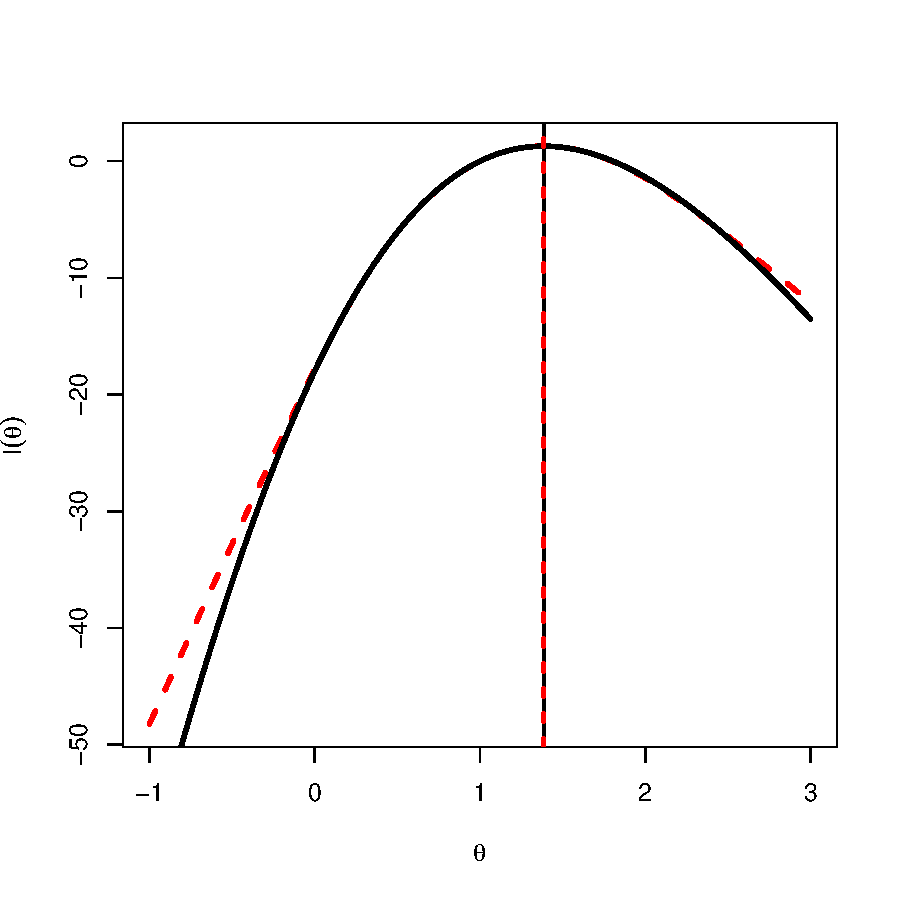
\includegraphics{sol10-010}

      We observe that the two curves are very close together in the region of the
      true MLE, and in fact the approximate MLE is very close to
      the true MLE in this case.
      \end{quotation}
      
      \item Try the same technique as in part (d) but use $\theta_0=0$. What do
      you observe?
      \begin{quotation}{\bf Solution:}
      Let us repeat most of the code from part (c):
\begin{Schunk}
\begin{Sinput}
> theta0 <- 0
> y <- rbinom(1e6, 100, exp(theta0)/(1+exp(theta0)))
> th <- seq(-1, 3, len=501)
> system.time(ellth <- sapply(th, ell))
\end{Sinput}
\begin{Soutput}
   user  system elapsed 
 15.536   1.245  16.787 
\end{Soutput}
\begin{Sinput}
> plot(th, ellth, type="l", lwd=3, lty=2, col=2, xlab=expression(theta),
+     ylab=expression(l(theta)))
> lines(th, (th-theta0)*xobs - 100*log((1+exp(th))/(1+exp(theta0))), lwd=3)
> abline(v=log(4), lwd=2)
\end{Sinput}
\end{Schunk}
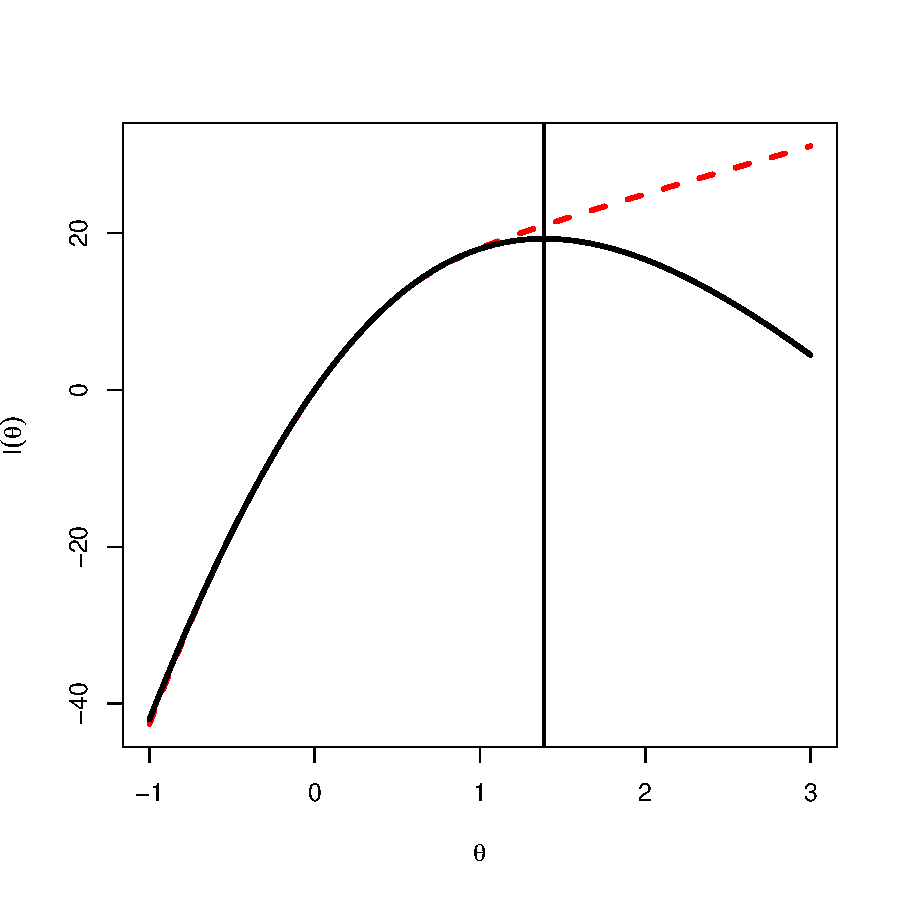
\includegraphics{sol10-011}

      In this case, the approximate (dashed red) curve is very close to the true
      curve in the neighborhood of $\theta_0$, but near the true MLE, this
      approximation breaks down and in fact, the approximate curve has no 
      maximizer at all in this case!
      \end{quotation}
      
    \end{enumerate}

\end{enumerate}

\end{document}

